\section{Introduction}
	\subsection{Motivation}
		\textit{Nuclear Magnetic Resonance} is a physical phenomenon that can be observed while placing an ensemble of nuclei into a static magnetic field and stimulate it with a high-frequent alterning field. A necessary condition for this effect is that the atoms of the sample have a \textit{nuclear spin} different from zero. It is the central concept that is used for \textit{NMR-Spectroscopy}, a standard methodology for the investigation of the structure and interaction of complex molecules and solid state bodies by measuring local magnetic fields, and the \textit{magnetic resonance tomography} which is an imaging technique used in clinical diagnistics for describing the morphilogic and physiologic build-up of tissues and organs. For all of those applications some important parameters of particular physical compensation-processes, the so called \textit{relaxation times} $T_1$ and $T_2$ need to be quantified. In the following experiment exactly those material-characteristic observables are determined for an ensemble of $^{57}$Fe-nuclei. But at first some basic knowledge.
	\subsection{Nuclear Zeeman-Effect}
		Every quantum mechanic angular momentum - especially every spin - is correlated with a magnetic moment $\mu$ The proportionality factor is called the \textit{gyromagnetic ratio} $\gamma$. So the intrinsic magnetic momentum matching to the nuclear spin $\vec{\mathcal{I}}$ considered in the experiment is given by:
			\begin{align}
				&\vec{\mu} = \gamma \vec{\mathcal{I}} \label{eq:mu}\\
				&\gamma  = g_I \frac{\mu_N}{\hbar} \overset{^{57}Fe}{=} 0.8661\cdot 10^{7}\ \unit{T^{-1}s^{-1}} \label{eq:gamma}
			\end{align}
		Where $\mu_N$ is the \textit{nuclear magneton} and $g_I$ is the Land\'{e}-factor which both are core-specific pa\-ra\-me\-ters. If those magnetic moments are placed in a static magnetic field $\vec{B} = B \vec{e}_z$ then the Hamiltonian of the system and its Eigenvalues to the Eigenstates of the spin-operator $\ket{I,m_I}$ are given by:
			\begin{align}
				&\mathcal{H} = - \vec{\mu} \vec{B} \overset{(\ref{eq:mu})}{=} - \gamma \mathcal{I}_zB \\
				&\langle\mathcal{H}\rangle = \bra{I,m_I}\mathcal{H}\ket{I,m_I} = -\gamma B \bra{I,m_I}\mathcal{I}_z\ket{I,m_I} = -\gamma B \hbar m_I \equiv E_{m_I}
			\end{align}
		Where the Eigenvalues of the Spin-operator for given spin-quantumnumber $I$ and magnetic quantum number $m_I = -I,\dots,I$ were used. So the outer magnetic field annuls the $2I+1$-fold degeneration of the energystates. The nuclear spin-quantum-number of $^{57}Fe$ is I = 1/2 so there are two additional energystates with a energydifference:
			\begin{equation}
				\Delta E = \hbar \gamma B = \hbar \omega_L \label{eq:lamor}
			\end{equation}
		As equation (\ref{eq:lamor}) suggests, there may occur optical transitions between the terms which lead to an emission of photons with the angular frenquency $w_L$. One finds that this frequency is equivalent to the \textit{Larmor-Frequency} that describes the precession of a magnetic moment around the z-axis caused by the torsional moment $\vec{M}=\vec{\mu}\times\vec{B}$ in a magnetic field. The classical description of this process leads to the same result as quantum mechanics do. If we consider the ensemble of $N$ nuclei as canonical, then the number of spins in the state $\ket{s,m_I}$ in the thermodynamic equivilibrium is given by the Boltzman-statistics:
			\begin{equation}
				N(m_I) = N \cdot \frac{e^{-\frac{E_{m_I}}{k_BT}}}{Z} = N \cdot \frac{e^{\frac{\hbar \gamma B m_I}{k_BT}}}{Z}
			\end{equation}
		Where $Z = \text{const.}$ is the canonical partition function and T is the absolute temperature of the environment. This implies that the spins prefer to be polarised not uniformely but in the direction of the B-field so this leads to a mean magnetic moment $\langle\vec{\mu}\rangle \neq 0$. This leads to an oberservable macroscopic magnetisation in the volume $V$:
			\begin{equation}
				\vec{M} = \frac{d\vec{\mu}}{dV} \cong \frac{N}{V} \langle\vec{\mu}\rangle \neq 0
			\end{equation}
		These changes in magnetisation are used to induce voltages that can be measured.
		
	\subsection{Hahn-spinecho} \label{int:secHahn}
		If the spins are just inside of a static magnetic field along the z-axis then they precess around this axis with an angular frequency of  $-\omega_L$. In the next step an alterning magnetic field $\vec{B}_{RF} = B_{RF}\sin(\omega t)\vec{e}_x$ is applied to the spins additionally. If we consider \textit{resonance} of the Larmor-precession and the radio-frequency field, i.e. $w = w_L$, then we can rotate the magnetisation around the x-axis by an angle of $\alpha = \gamma B_{RF}t$ where t is the time the RF-field is applied. With this effect we can now apply different \textit{magnetic resonance sequences} to investigate the interaction of the spins with each other and the external magnetic fields.\\
		The first sequence is a really simple one: the $90 \unit{°}$-pulse where the spins are flipped in the xy-plane, i.e. $\vec{M} \perp B\vec{e}_z$. Because they now rotate around the z-axis in the laboratory system the periodic change of the magnetic field within the coil that is part of the HF-circuit leads to the induction of an alterning voltage with frequency $\omega_L$. Because the spin-moments interact with each other their angular frequency differs from spin to spin. This Dephasing leads to the decrease of the mean magnetisation in xy-plane and so the measured voltage fades away. This effec is called \textit{Free Induction Decay}. By applying an $180\unit{°}$-pulse after a time $\tau$ the spins rephase and the voltage increases again (\textit{Hahn-Spinecho}). Because of irreversible effects during de- and refocussing the polarisation decreases and the mean magnetisation in xy-plane and the measured voltage have a lower amplitude. The correlation between the dephasing time $\tau$ and the mean magnetisation in xy-plane can be described by an exponentially decaying function:
		\begin{equation}
			U_{ind}(\tau) \propto M_{xy}(\tau) = M_{xy}(\tau = 0) \cdot e^{-\frac{2\tau}{T_2}}
		\end{equation} 
		The decay of the reversible nuclear magnetisation is called \textit{spin-spin-relaxation} and the corresponding time constant is the \textit{spin-spin-relaxationtime} $T_2$. In the experiment it will be measured by variing $\tau$ and measuring the alterning voltage $U_{ind}$. Figure (\ref{int:t2}) depicts the Hahn-Spinecho.
		\begin{figure}[h]
			\centering
			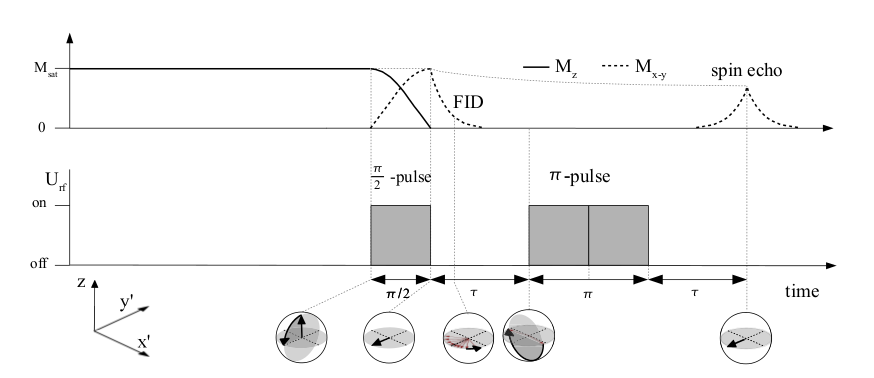
\includegraphics[scale = 0.4]{pic/intro_t2}
			\caption{Hahn-Spinecho sequence for measuring $T_2$ relaxation time}
			\label{int:t2}
		\end{figure}
	\subsection{Spin-Latice Relaxation}
		Because the energy of an ensemble of spins is minimal when they are polarised longitudinally along the magnetic field $B\vec{e}_z$ they are into they will relax to this equivilibrium state when it is perturbed, e.g. by a 90°-pulse. After applying this pulse and waiting for a time $\Delta t$ the z-component of the mean magnetic moment $\langle \mu_z \rangle$ increases. After $Delta t$ a Hahn-Spin-echo sequence mentioned in section (\ref{int:secHahn}) is applied.  Because the measure signal of this sequence is proportional to the initial magnetisation we will induce an echo-voltage in the HF-coil that increases by waiting longer after the 90°-pulse such that more spins are relaxed back to the equivilibrium state. The dependency between $\Delta t$ and the measure signal can be described by:
		\begin{equation}
			U_{ind}(\Delta t) \propto M_{xy}(\Delta t) = M_{sat} \cdot [1-e^{\frac{\Delta t}{T_1}}]
		\end{equation}
		The relaxation of the longitudinal component of the magnetisation is called \textit{Spin-latice relaxation}. The occuring time constant $T_1$ is the \textit{Spin-latice-relaxation time} and corresponds to the time one has to wait between the pulses such that the magnetisation is approximately $63.21\ \unit{\%}$ of the saturation value. This parameter will be measured by variing $\Delta t$ and holding the time-constant of the Hahn-sequence $\tau$ constant. Figure (\ref{int:t1}) depicts the sequence.
		
		\begin{figure}[h]
					\centering
					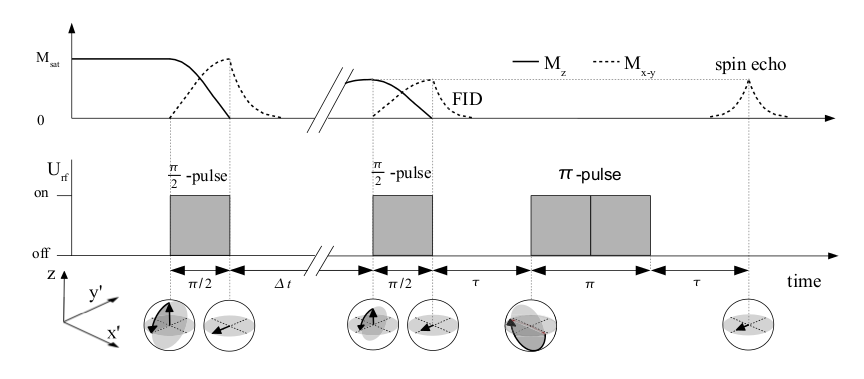
\includegraphics[scale = 0.4]{pic/intro_t1}
					\caption{MR-sequence for measuring the spin-latice relaxation time $T_1$}
					\label{int:t1}
		\end{figure}